
\section{Parallelizing Datalog on the GPU}
%
Programmable GPUs provide massive fine-grained parallelism, higher raw computational throughput, 
and higher memory bandwidth compared with multi-core CPUs. As a result they are a favorable  
alternative over traditional CPUs when it comes to high throughput implementations of applications.
GPU implementations can potentially provide several orders of magnitude in performance 
improvement over traditional CPUs. As a result, GPU technology is increasingly widespread
and has been successfully adopted by significant number of data-intensive
scientific applications such as molecular dynamics~\cite{ANDERSON20085342}, physical simulations~\cite{EGVE:IPT_EGVE2005:105-111},
and ray tracing in graphics~\cite{Parker:2010:OGP:1833349.1778803}.

\subsection{GPU architecture}
\begin{wrapfigure}{R}{0.45\textwidth}
	\centering
	\vspace{-0.1in}
	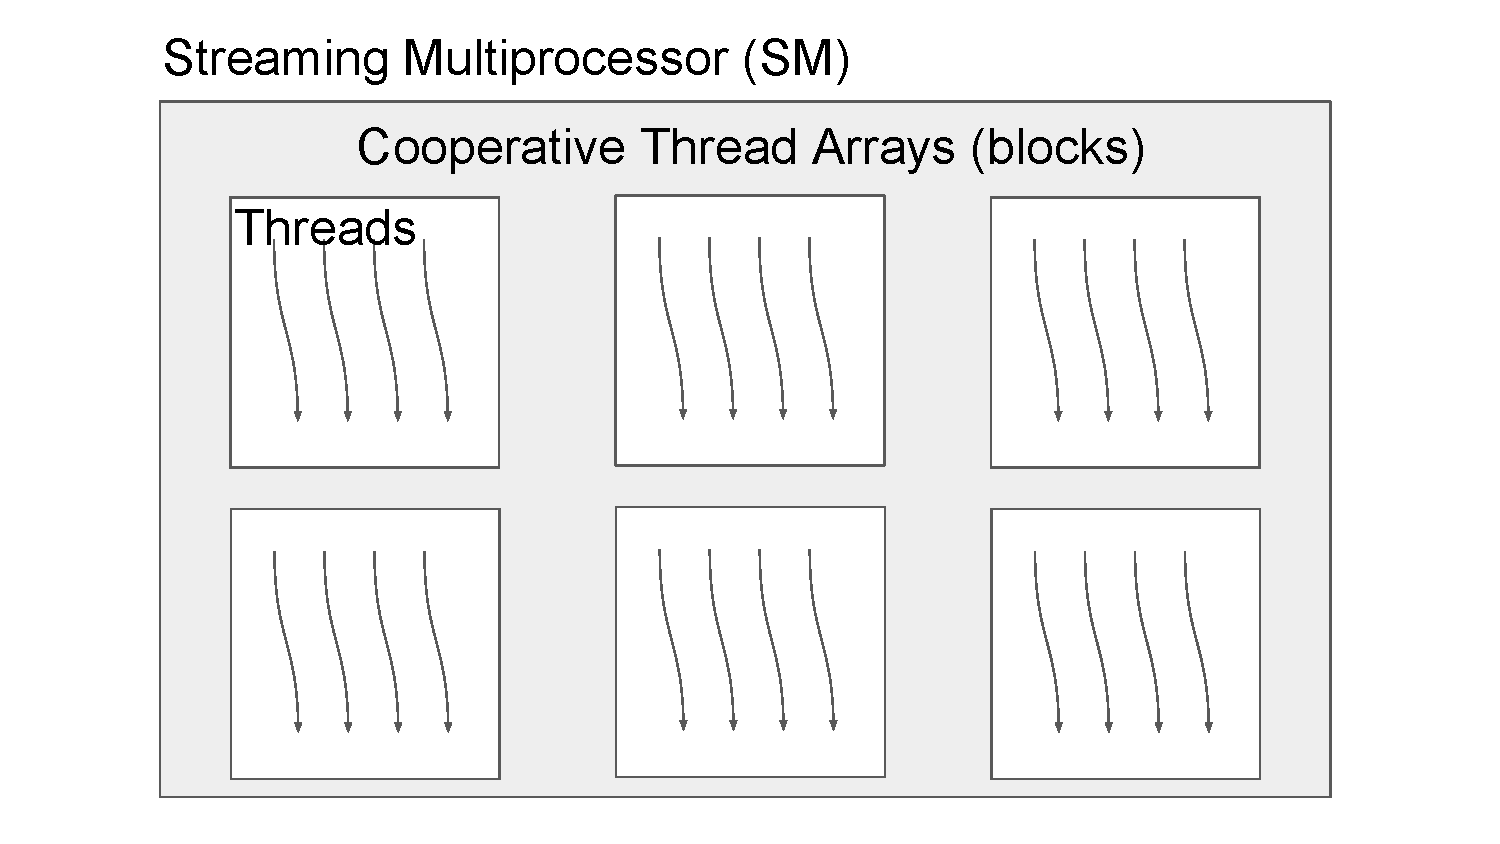
\includegraphics[width=.99\linewidth]{GPU.pdf}
	\caption{High-level overview of GPU. \label{fig:gpu}}
	\vspace{-0.2in}
\end{wrapfigure}

Threads provide the finest level of parallelism in a GPU.
A GPU application is composed of a series of multi-threaded data-parallel kernels. 
Data-parallel kernels are composed of a grid of parallel work-units called Cooperative Thread Arrays
(CTAs) which in turn consist of an array of threads. In such processors, threads within a CTA are grouped into logical units
known as warps that are mapped to SIMD units called Stream Multiprocessors (SMs) (see Figure~\ref{fig:gpu}).
The programmer divides work into threads, threads map to thread blocks (CTAs), and thread blocks map to a grid. 
The compute work distributor allocates thread blocks to SMs. 
Once a thread block is distributed to an SM the resources for the thread block are allocated 
(warps and shared memory) and threads are divided into groups of (typically) 32 threads called warps. 


\subsection{Redfox}
We use Redfox~\cite{Wu:2014:RFE:2581122.2544166} a GPU-based open-source tool to run the relational algebra (RA) kernels translated from Datalog.
Redfox is used for compiling and executing queries expressed in a specialized query language on GPUs.
Typically, the parallelism involved in solving relational-algebra operations on GPUs is challenging due to 
unstructured and irregular data access as opposed to other domain-specific operations, such as those
common to dense linear algebra. 
Redfox tackles these issues and provides an ecosystem to accelerate relational computation including
algorithm design, system implementation, and compiler optimizations. It bridges the semantic gap 
between relational queries and GPU execution models, allowing its clients to operate exclusively in terms of
RA semantics, and maintains significant performance speedup relative to the baseline CPU implementation. 

Redfox takes advantage of the fine-grained massive parallelism offered by GPUs.
It is comprised of (a) a specialized language front-end that allows the specification of sequences of RA operations
that combine to form a query, 
(b) an RA to GPU compiler, (c) an optimized GPU implementation of select RA operators, and (d) a supporting runtime.
The relational data is stored as a key-value store to support a range of workloads corresponding to queries over data
sets. We use our own system to transform datalog queries into RA kernels. Redfox provides a GPU implementation of
the following set operations:  union, intersection, difference, cross product, inner-join, project and select. Among all
the RA primitive operators,
inner-join is the most complex and is more compute intensive than the rest of the RA primitives. Another 
problem with joins is that their output size can vary, i.e. between zero to the product of the sizes of the two inputs.
One of the salient contributions of redfox is an optimal implementation of the join operation~\cite{wu_adms14}.

\subsection{Fixed-point iterations with Redfox}
\begin{wrapfigure}{R}{0.45\textwidth}
	\centering
	\vspace{-0.1in}
	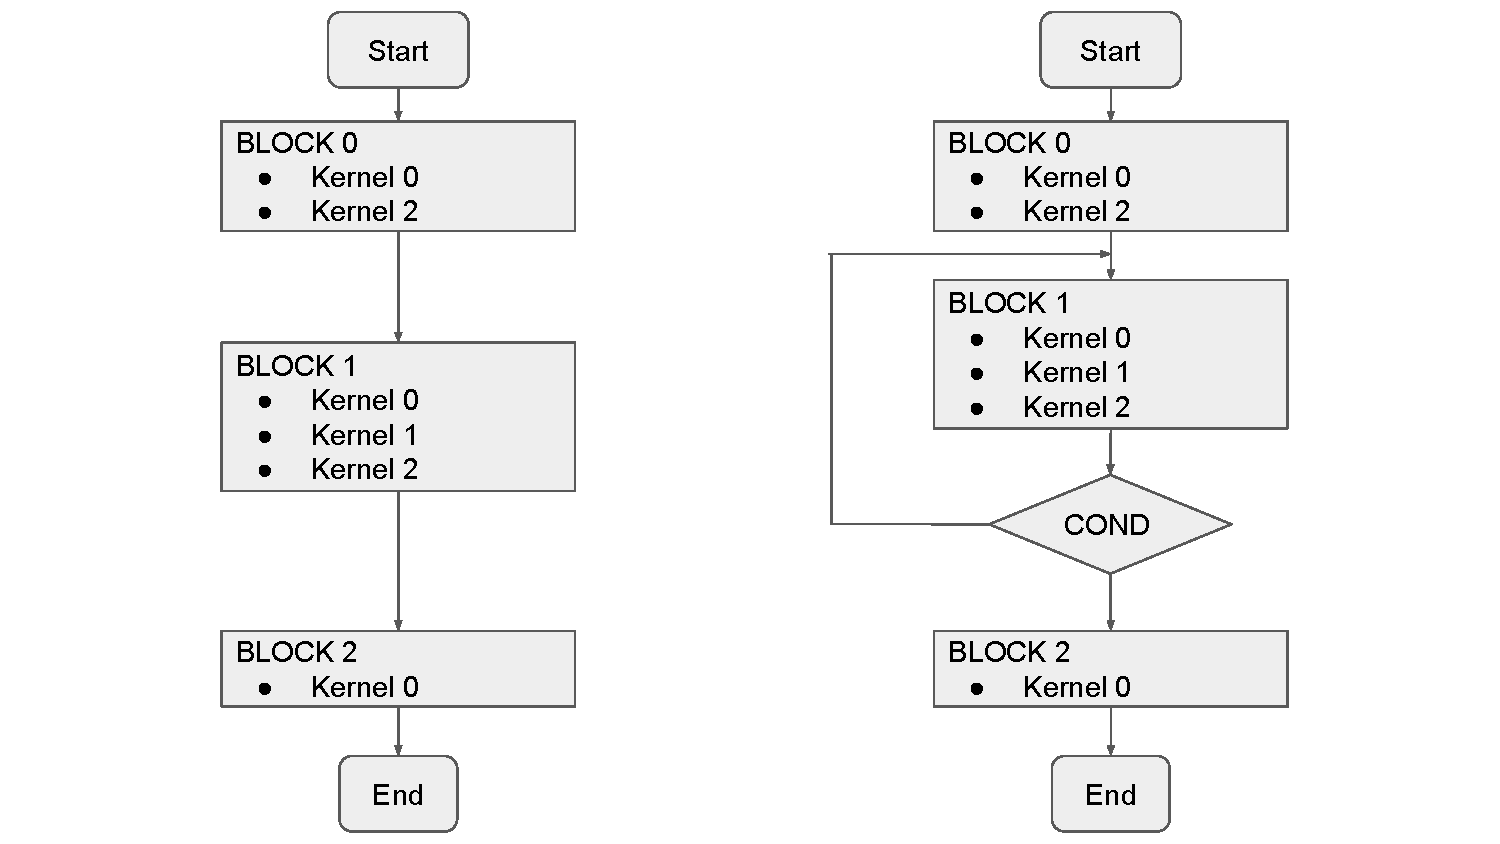
\includegraphics[width=.99\linewidth]{redfox-brances.pdf}
\caption{Redfox execution with (right) and without (left) conditional branches. \label{fig:scale}}
\vspace{-0.2in}
\end{wrapfigure}

One of the major challenges in adapting redfox to solve RA kernels derived from datalog
queries was to perform fixed-point iterations. For fixed-point iterations redfox needed to process loops and, until now, Redfox
was only used in a sequential mode, where a block unconditionally transitioned to the next block. In the original Redfox paper's experiments, the authors did use a fixed-point computation, but had manually unrolled the benchmark to the needed number of iterations. In our application,
we need the ability to run basic blocks (each a straight-line sequence of RA kernels), in a loop, until the 
relation in contention does not change and the system reaches a fixed point---regardless of how many loops this requires. 
In order to facilitate execution of loops in redfox, we have added conditional branches, that allows execution to choose a target basic block based on the equality of two input relations. We used the COND kernel of GPU and use the outcome of the kernel to schedule the target block. 
Typically, in fixed-point iterations we check if the values stored in relation after execution of a certain kernel changed or not, if it remains unchanged then
we have attained a fixed point and the execution can move forward, otherwise the set of kernel is executed again (see Figure~\ref{fig:scale}).


\subsection{Preliminary results}
%
We evaluated the performance of Redfox in computing the transitive closure of large-sized graphs. 
For benchmarking we used the open source graphs available at~\cite{UF:SPMC}.
Out of all relation operations used in computing the transitive closure, join is computationally the most complex.
We found that the join operation manage to scale decently well with larger graphs.
Time consumed performing join operation across 188 iterations
for input graph of 25,674 edges (output size is 6,489,757 edges) took 3.6 seconds. Total time for other kernel operation (project, union, copy) along with I/O time was 3.3 seconds. This total time (3.6 + 3.3 seconds) is almost comparable to the time taken by the highly optimized code Souffle (5.6 seconds) to compute the transitive closure of the same graph. We surmise, that Souffle is able to extract parallelism sufficient enough to solve the problem for this graph. Our hypothesis is that the GPU performance may become significantly faster than Souffle for very large scale graphs.




